\documentclass[cn,11pt,twocol,table]{elegantbook}
\usepackage{fontawesome5,booktabs,listings,metalogo,colortbl,tabularx,pifont}
\usepackage{amssymb}
\PassOptionsToPackage{table}{xcolor}
\usetikzlibrary{patterns}

\newcommand\link[1]{\href{#1}{链接\faLink}}
\newfontfamily\libertinus{Arial}
\setCJKfamilyfont{hei}{SimHei}
\newcounter{tblerows}
\expandafter\let\csname c@tblerows\endcsname\rownum

\title{使用\LaTeX{} 做Beamer踩坑记}
\subtitle{掉头发之旅}

\author{Will}
\institute{University of Manchester}
\date{\today}
\version{0.01}

\extrainfo{子曰:will子真乃学习狂人也}

\logo{logo.png}
\cover{cover.jpg}

\begin{document}
\maketitle
\tableofcontents
	
\mainmatter
\hypersetup{pageanchor=true}	
\chapter{字体}
\label{ch-1}
\begin{introduction}
\item 字体是\LaTeX{} 学习过程中不能逾越的一条沟!
\item 不要相信csdn、百度、知乎上的大部分回答
\item 尽量使用英文搜索
\end{introduction}	

\section{字体设置}
大多数使用\LaTeX{} 进行文章、书籍、Beamer创作的人肯定不是因为其方便易用(绝对不是!!),大多数人是因为\LaTeX{} 所产出的文件排版美观(当然得首先选择美观的模版(theme, template))。由此看来,世上颜值党多矣!\par
既然是因为顔值,那就需要考虑很多的因素:字体搭配、颜色搭配、版面设计……
\begin{note}
在没有一定的基础知识与\emph{审美}之前,不要尝试自己从零开始做一个自己认为的美观模版\footnote{鄙人曾于天朝逼乎上见到过一位“高手”展示自己使用\LaTeX{} 排版的结果,让人不敢苟同。}。\par
\end{note}
在安装了Texllive 2019之后,字体的设置就相当的简单。只要按照正常的字体安装流程安装自己喜欢的字体即可。
\begin{note}
	Win10 \faWindows 的字体安装可能与Win7有所不同。在Win10下安装字体需要选择 install for all users才能正常被Texlive调用。 切记!吾曾于此坑中耗费一时辰光阴。
\end{note}
\subsection{常用的字体相关宏包推荐}
刚刚讲过,世上多顔值党,而\TeX{} buildin template又实在是难入吾辈顔值一党法眼。并且\TeX 与\LaTeX 其原作大神尤钟爱“简洁”、“素净”的排版风格,实在是不够优雅。 于是使用一系列宏包(package)增加一些风格化的设置成为必要。推荐表\ref{tab-1}中的宏包:
\begin{table}[htbp]
\centering
\begin{tabular}{lll}
	\toprule
	宏包&作用&原包链接\footnotemark\\
	\midrule
	fontspec&对文章中的字族进行设置&\link{https://ctan.org/pkg/fontspec?lang=en}\\
	pifont&包含各种符号的宏包&\link{https://ctan.org/pkg/pifont?lang=en}\\
	fontawesome5&可以提供各种图标的宏包(配合手册使用效果更佳)&\link{https://ctan.org/pkg/fontawesome}\\
	\bottomrule
\end{tabular}
\caption{常用字体宏包推荐}
\label{tab-1}
\end{table}
\footnotetext{伟批:考证!似乎并无原包链接此词}
\subsection{fontspec宏包使用}
fontspec宏包最常见的用法是为文档类设置rmfamily、sffamily以及ttfamily。使用方法如下:
\begin{lstlisting}[language=TeX]
%导言区(文档类开头)使用fontspec宏包
\usepackage{fontspec}
\setmainfont[<Options>]{<Font name>}
\setsansfont[<Options>]{<Font name>}
\setmonofont[<Options>]{<Font name>}
%设置字体时的选项后面会介绍到
\end{lstlisting}
以上三项分别对应rmfamily、sffamily以及ttfamily。fontspec可以自动找到对应字体的粗体、斜体等其它字体的变体。关于字体的更多相关介绍可以参考于海洋出版的《\LaTeX{} 入门》\footnote{此书可以随时多查看几遍,非常有利于新手入门}。
\subsubsection{fontspec字体选择}
fontspec宏包选择字体([<font name>])有两种方式:\emph{以字体名}和\emph{以字体文件名}。但是江湖上似乎更加偏向以字体名引用字体,对另一流派往往并不提及。\par
\paragraph{字体名选择}
以字体名选择实在简单,只要在正确的位置写入正确的字体名称即可。然曾有圣人言,大问题多起于微末。正确的字体名字往往是很多新入门同学遇到的第一个问题。提供一个方便可靠的方法。Windows系统,在CMD中执行fc-list > fontlist.txt 指令,可以生成本机上所有字体的名称\footnote{生成的fontlist.txt文件位于C:$\backslash$user$\backslash$*username*文件夹下}。\par 
Win10用户安装字体时,请注意使用install for all users。\par
以字体名选择的方式,可以自动查找匹配此字体名下的bold以及italic字体,并且使得\lstinline|\textbf|与\lstinline|\textit|即时生效。
\paragraph{字体文件名选择}
\XeTeX 与Lua\TeX{} 同样也支持使用字体文件名来引用字体。根目录下的字体文件可以不用声明文件路径而直接引用。与字体名引用时自动匹配bold与italic不同,使用字体文件名引用时,必须要声明bold与italic字体名(文件名)。同样给一个粟子:
\begin{lstlisting}[language=TeX]
\setmainfont{SourceHanSerifSC-regular.otf}[
BoldFont=SourceHanSerifSC-Bold.otf,
ItalicFont=SourceHanSerifSC-italic.otf,
...]
\end{lstlisting}
如果觉得重复写文件扩展名和文件名不够优雅,也可以使用下面的简写代码:
\begin{lstlisting}[language=Tex]
\setmainfont{SourceHanSerifSC}[
Path =/User/Will/Fonts/, %此处需根据自己具体的字体文件所在写路径
Extension=.otf,
UprightFont=*-regular, %注意此处需要声明regular文件
BoldFont=*-Bold.otf,
ItalicFont=*-italic,
RawFeature=+fwid
...]
\end{lstlisting}
有时候你会发现一些高手的文档定义中,会对UprightFont, BoldFont, ItalicFont等进行重新的映射以获得更加细致的调整。在一些文档中,你还有可能发现RawFeature这个选项\footnote{详细的可用选项见https://docs.microsoft.com/en-us/typography/opentype/otspec140/featurelist},此选项是对opentype字体的一些调整。
\subsubsection{数学公式字体选择}
此部分内容不完全\par
出于优雅的需要,数学公式或者数环境下的字体往往是不同的,但是一些数学相关字体\lstinline|\mathrm|等默认与正文字体一致。当使用fontspec设置正文字体的时候,就会受到影响\footnote{\LaTeX{}下浩如烟海的宏包以及莫名其妙地不同宏包之间的冲突,使得K公当年内容格式分离的想法变的滑稽可笑。此事按下不表。}。此时我们有两种方法:
\begin{itemize}
	\item 使用\lstinline|\setmathrm{<Font Name>}|等命令对数学字体进行定义。
	\item 使用 no-math 宏包选项声明不对数学环境生效\footnote{大多数数学宏包已经默认执行此指令}
\end{itemize}
\section{中英开源字体推荐}
英文: LibertinusSerif\par
中文: 思源宋体\par
本文中的使用的宋体即为思源宋体,正文中的英文为Libertinus。(后面会补充更多的字体搭配,以实现多元化的选择)

\chapter{版面设计}
\begin{introduction}
\item 分栏
\item 图片
\item 表格
\end{introduction}
Will本人是一个PPT重度用户,从研究生时就开始自己设计PPT模版、动画\footnote{著有伟哥PPT模版练习,仅发布于Will的个人电脑硬盘}。在PPT中(或者可以说所有的演示类文档)中最为重要的就是版式:是全页大图,还图文混排?是上下结构,还是左右结构?左右结构又采用什么样的构图?一众问题都有非常专业的设计人员在思考、研究。 \par
在\LaTeX{} 或者说Beamer中如果要自由地实现上述所有要求,那非常傻的。\LaTeX{} 的设计就决定了用户层面与后台设计层面的巨大鸿沟!想一个人既完成前端内容,又完成后台样式实现需要花费相当的时间成本。古人曾言,术业有专攻\footnote{出版韩愈《师说》,闻道有先后,术业有专攻。},Will认为,吾辈切莫有“工具优越感”,认为\LaTeX{} 就要比其它的工具优秀。大多数情况下,\LaTeX{} 在易用性、源文件可读性上要远远不如PPT、Word等工具。 曾有人做出过如下的总结,Will深以为是:
\begin{quote}
不会用\LaTeX{} :编译错误,得不到文档\par
不会用Word:难看的文档\par
会用\LaTeX{} :好看的文档\par
会用Word:一般的文档\par
精通\LaTeX{} :精美的文档\par
精通Word:精美的文档
\end{quote}
足见这两种工具并不存在某种工具更优秀,在学习新的工具的时候一定要认清工具的局限与长处。
\section{分栏}
分栏在文章投稿和PPT中尤其常见,在文章投稿中比较固定,但是在PPT中则显的尤为重要。因此本章的分栏主要讲解Beamer下的实现。在PPT中其实就是版式设计,如前面所言,众多设计人员精于此道。所以在\LaTeX{} 我们只需要知道如何实现别人设计好的版式即可。\par 
\subsection{分栏的实现}
在演示文稿中要实现图文混排,多数情况是需要用到分栏工具。在Beamer 中使用\lstinline|\begin{columons}|开启分栏。在此环境下,再使用\lstinline|\begin{column}|即可增加一栏。详细的使用如下例:
\begin{lstlisting}[language=TeX]
\documentclass{beamer}
...
\begin{document}
\begin{frame}
\frametitle{Nuclear Propulsion} %Beamer 标题
\begin{columns}
\begin{column}[T]{0.48\textwidth} %设置对齐方式以及宽度
\vspace{0pt}%
\includegraphics[width=\columnwidth]{AtomicSubmarine}
\vspace{1em}
\tiny
\begin{enumerate}
\item Item1$\rightarrow$ Conclusdion
\item Item2$\rightarrow$ Conclusdion
\item Item3$\rightarrow$ Conclusdion
\end{enumerate}
\end{column}\hfill %\hfill实现左右两栏的水平分布
\begin{column}[T]{0.48\textwidth}
\includegraphics[width=0.9\columnwidth]{SubmarineSnorkel}
\end{column}
\end{columns}
\end{frame}
\end{document}
\end{lstlisting}
如果要实现一些修改,环境的选项[<options>]则非常重要,在columns环境中,有如下的选项可供使用:
\begin{description}
	\item[b] 不同的分栏之间底对齐
	\item[c] 不同的分栏之间中心对齐
	\item[onlytextwidth] 设置分栏的总宽度为beamer页面版心宽度(防此内容超出页面)
	\item[t] 不同分栏之间第一行对齐(类似于项端对齐)
	\item[T] 与t类似,但T对齐的是第一行的top,而t对齐baseline,如果在t模式下出现图片排版问题,可以尝试使用T模式。
\end{description}
此处修改不同的column width就可以实现你相中的版式设计。具体哪种比例好看,那就因人而异了……
\subsection{分栏中可能遇到的问题}
在PPT中我们可以随心所欲地安排任意对象的位置大小比例,但是在Beamer下则显的有些困难。这里Will列举一些自己在Beamer制作过程中遇到的问题以及可能的解决方法。如果有更好的建议,请\href{mailto:liweicfd@hotmail.com}{邮件}告知本人。
\paragraph*{分栏中某一栏垂直分布}
此问题常见于两栏中有一栏的内容比较少,不能填满垂直空间,通常Will对此类问题在PPT下就是垂直分布,不至于显得PPT中有某一块太空。而columns环境提供的顶部对齐,中心对齐以及底部对齐不能满足设计美观的需要。对此可以使用\lstinline|\vfill|来实现弹性填充,垂直分布。\par
但是理想是丰满的,现实总是骨感的\footnote{伟批:未知出处}。直接使用\lstinline|\vfill|就会发现,此命令好像没有起作用,布局没有发生任何的变化。搜索之后发现这样一则帖子:
\begin{quote}
	The \textit{column} environment is using a \textit{minipage} environment internally which doesn't has a predefined height like the whole frame has. The \lstinline|\vfill| macro fills out the rest of given the vertical space. Because there is no height defined it does nothing. You have to define the height\footnote{\link{https://tex.stackexchange.com/questions/15244/why-does-vfill-not-work-inside-a-beamer-column}}.
\end{quote}
根据此解释,Beamer中的column是使用minipage机制实现的,但是并没有预定义高度,而\lstinline|\vfill|则是需要根据所在环境的高度进行弹性填充。所以在column中vfill无效果。\par
解决这个问题的方法就是使用一个minipage定义column的高度\footnote{伟批:Will深感些方法之不优雅}。解决方法可参照下例:
\begin{lstlisting}
\documentclass{beamer}
\begin{document}
	\begin{frame}{foo}{bar}
		\begin{columns}[t]
			\begin{column}{\textwidth}
			\minipage[c][0.7\textheight][s]{\columnwidth} %在此处使用minipage定义高度
			Blublub
			\vfill
			Blablabla
			Blublub
			\vfill
			Blablabla
			\endminipage
			\end{column}
		\end{columns}
	\end{frame}
\end{document}
\end{lstlisting}
\subsection{Frame尺寸、边距设置}
frame是Beamer中一张slide的名称,设置Frame的尺寸和边距同样是我们获得优雅好看的PPT中极重要的一环。
\subsection{背景}
想好看嘛?想就加上一张有设计感、高级感的背景。
\section{表格\&图片\&列表}
版式完成之后,我们要做的事情就比较简单了,把正确的内容添加到正确的位置。考虑到“美观”与“优雅”\footnote{已经不知道说了多少次优雅这个词了……},绝大多数情况下,我们需要对插入的表格、图片、列表进行一系列的调整,以达到听众友好(误……这里就需要考虑到一些PPT制作的要点比如:
\begin{itemize}
	\item 一页PPT最好只讲述一个问题点
	\item 注意视觉重点引导
	\item 使用排版,而不是动画来安排过多内容
	\item 注意版面利用率,不要有大片空白与拥挤
	\ldots
\end{itemize}
\par
对PPT设计感兴趣的同学可以自行去找一些文章读读看,也是相当大的一个坑\footnote{就方便上手与最终效果方面,私以为PPT完胜Beamer,觉大多数上来就说\LaTeX{} 要比Office套件好的人应该是很少或者没有考虑过Office应该如何使用。在2019年的当下,Office套件的方便与人性化程度实在不知道比\LaTeX{} 高到哪里去了。}。 这些要点对任何演讲稿都是普遍适用的,在Beamer中我们同样需要遵循这些要点。而在科研方向上,对表格、图片与列表的整齐、简洁、明了则更加重视。毕竟我们在台上说着不流利的英语的时候,台下的大佬们已经昏昏欲睡,他们不仅要忍受着难听的口音,抵抗着睡虫的干扰还要在你讲完之后,给你提出“合理化”的建议。所以即使从人道主义的角度出发,我们也应该给他们看一个重点清晰、能一眼看懂你要说什么的讲稿。
\subsection{表格}
科研方向上对于表格的处理比较单一,往往是要求三线表的样式。如果你哪天看到谁给出一个五颜六色并且带着各种表格线的表,那基本上你可以放心大胆的给他提问题,放心,他答不上来的。表格常用到的宏包列于\ref{tab2-2}中:
%\rowcolors{3}{blue!50}{yellow!60}
\begin{table}[!hbtp]
%\centering
\rowcolors{1}{white}{blue!10}
\begin{tabularx}{\textwidth}{lXl}
\showrowcolors
\toprule
宏包&说明&链接\\
\midrule
array&array宏包扩展了array与tabular环境,增强了列样式的选项,可以改变列宽,使用编程命令定义新的样式等&\link{https://ctan.org/pkg/array?lang=en}\\
booktabs&booktabs宏包提供了三线表的命令,并且也提供了长表格的支持&\link{https://ctan.org/pkg/booktabs?lang=en}\\
tabularx&此包实现了表格整体宽度固定,列宽自动调整的功能&\link{https://ctan.org/pkg/tabularx}\\
colortbl&可以实现行、列、单元格以及表格线的上色&\link{https://ctan.org/pkg/colortbl}\\
xcolor&非常强大的颜色扩展宏包,其中的rowcolors可以在colorbl支持下实现奇偶行上色&\link{https://ctan.org/pkg/xcolor}\\
\bottomrule
\hiderowcolors
\end{tabularx}
\caption{表格相关宏包推荐}
\label{tab2-2}
\end{table}
\par
 %\hiderowcolors
其实说也来是辛酸,在Word或者PPT中看似非常简单,点几下鼠标就可以实现的功能,在\LaTeX{} 却需要引入众多宏包来实现\footnote{\LaTeX{} 的一个问题就是众多宏包,很多用户根本不知道有没有以及要用哪个宏包}。 Anyway,有了这几个宏包之后,我们就可以方便的调整表格了。\par
\begin{note}
在使用xcolor宏包时有可能会遇到几个问题,其中一个就是\textit{Option clash for package xcolor}。一旦遇到这个报错,那就说明你使用的其它宏包也调用了xcolor,并且调用位置在你调用之前。解决这个问题有两种方法:\par
\begin{itemize}
	\item 使用\lstinline|\PassOptionsToPackage|,将你需要的参数传递给已经调用的xcolor包。
	\item 如果能够找到是哪一个包调用的,可以手动调换package调用位置
\end{itemize}
\end{note}
\paragraph*{科学图表线型}
科学表格一般指三线表,所以只要使用booktabs宏包即可实现。使用方法非常简单。如果想自己指定线宽可以使用\lstinline|\toprule[width]|命令。
\begin{lstlisting}[language=TeX]
\usepackage{booktabs} %导言区引用宏包
\begin{table}
	\begin{tabular}{lll}
		\toprule	%插入第一条线 
		样品&模量&硬度\\
		\midrule	%插入中间横线
		c-121&250&3.1\\
		\bottomrule %插入底部横线
	\end{tabular}
\end{table}
\end{lstlisting}

\paragraph*{图表单双行颜色}
就在我写着写着,想着试验一下上面表格中的宏包,整个小例子的时候,发生了一个非常令人难受的bug:我使用\lstinline|\rowcolors|时,发现tabularx环境不变色,但是tabular可以正常变色…… 后面搜索到了别人相同的问题\link{https://tex.stackexchange.com/questions/297345/why-is-the-start-row-of-rowcolors-ignored-in-tabularx}。回答这个问题的是tabularx包的作者Carlisle,据Carlisle所述,这个问题是由于\TeX{} 中记数器没有正常重置有关\footnote{到底如何有关,我是没看明白\faSadTear[regular]},重置之后就可以解决。
\begin{lstlisting}[language=TeX]
%导言区加入这两句话
\newcounter{tblerows}
\expandafter\let\csname c@tblerows\endcsname\rownum
\end{lstlisting}

另外,我还发现一个小问题,如果想让tabularx正常的开启、关闭变色,需要在tabularx环境内再写一句\lstinline|\showrowcolors|才能正常开启。不知道是否是这两个宏包之间冲突。总之使用时要小心,并且做好耐心debug的工作\footnote{江湖传言,使用\LaTeX{} 写作十分钟,找错两小时。诚不我欺。}。\par
好了,吐槽结束,来讲一下如何实现表格奇偶不同色,主要下基于colortbl宏包与xcolor宏包下的rowcolors命令。在使用\lstinline|\rowcolors|命令时,要注意给xcolor宏包[table]选项。效果展示见\ref{tbl-color}\footnote{伟批:尽量不要搞一些太Smart的配色……}
\begin{lstlisting}{language=TeX}
\usepackage{colortbl}
\usepackage[table]{xcolor} %注意给出[table]选项
\begin{table}[htbp]
\begin{tabular}{1>{\columncolor{cyan}}11}
\rowcolor{blue!25}第一列&第二列&第三列\\ 
21&22&23\\
\end{tabular}
\end{table}
\end{lstlisting}
\begin{figure}[h]
\centering
\begin{tabular}{l>{\columncolor{cyan}}ll}
	\hline
	\rowcolor{blue!25}第一列&第二列&第三列\\ 
			21&22&23\\
		\hline
\end{tabular}
\caption{表格上色}
\label{tbl-color}
\end{figure}
\subsection{图片}
\LaTeX{} 的插图绝对是非常令人抓狂的一件事情,由于其不能实时调整,每次调整都需要不断的编译$\to$查看$\to$编译……如果是使用别人的模板,一切按照模板上示例图片的尺寸来搞,可能还好一点,一旦自己的图片与模板不一致,后面调整起来真的费事。\par
在\LaTeX{} 插入图片可使用graphicx宏包提供的\lstinline|\includegraphics[code]{imagefile}|命令。此命令可以接收参数,从而一定程度上调整插入的图片的样式。具体的参数说明请见表\ref{tab-img}
\begin{table}[h]
	\begin{tabularx}{\textwidth}{lX}
		\toprule
		参数&说明\\
		\midrule
		width=x,height=y&设定图片的宽与高,可以使用任意长度单位。\\
		scale=s&设置图片的缩放比例,与上一行中的宽高设置任意采用一种使用,同时使用时,绝对尺寸有效\\
		keepaspectratio&保持缩放比例\\
		angle=a&旋转角度设置\\
		origin=hv&水平与垂直方向上的旋转中心,分别可以选择l,c,r与t,c,b\\
		page&选页,在插入pdf这类有多页的图片文件时,可以选页\\
		\bottomrule
	\end{tabularx}
\caption{$\backslash$includegraphics[code]{imagefile}参数说明}
\label{tab-img}
\end{table}

\paragraph*{图片对齐方向}
图片的对齐一般最常用的就是centering居中对齐,但是在极少数的情况下,可能会有同学要用到一些非常奇怪的对齐方式,比如左对齐与右对齐等。推荐直接使用ragged2e宏包提供的各种命令,相比\TeX{} 原本的\lstinline|\raggedleft|等命令可以得到更加合理的段落\link{https://ctan.org/pkg/ragged2e?lang=en}。
\begin{note}
	当我们插入figure环境的时候,figure默认的尺寸是textwidth,但是caption是默认在textwidth中间位置对齐,所以当你使用了其它方式对齐图片的时候,会发现一个问题:图片的caption不会对齐到图片的中间位置。
\end{note}

\paragraph*{图片标注}
很多时候,我们在做PPT的时候,需要对图片进行标注,让听众(老板!!)知道我们在讲什么地方。在PowerPoint中,这似乎从来不是问题,但是在\LaTeX{} 中这就是一个比较麻烦的事情。当然我们可以对图片先进行标注,做出标注之后的图片,再插入到文档中,但是这一点也不够优雅\footnote{又一次讲优雅!}!还有一种方法就是使用Tikz宏包对图片进行标注。说成大白话就是用命令来画我们需要的标注框、箭头、标签等\footnote{伟批:这种方法听起来更加中二,纯粹无聊的炫技。}……\par
既然都要学习使用\LaTeX{} 了,那怎么也得学习下如何使用Tikz宏包来画图。假如我想在图\ref{fig:exam}中的红黑两条线古画一个虚线框,将其作为一组来重点讲述,那应该如何是好呢?
\begin{figure}
	\centering
	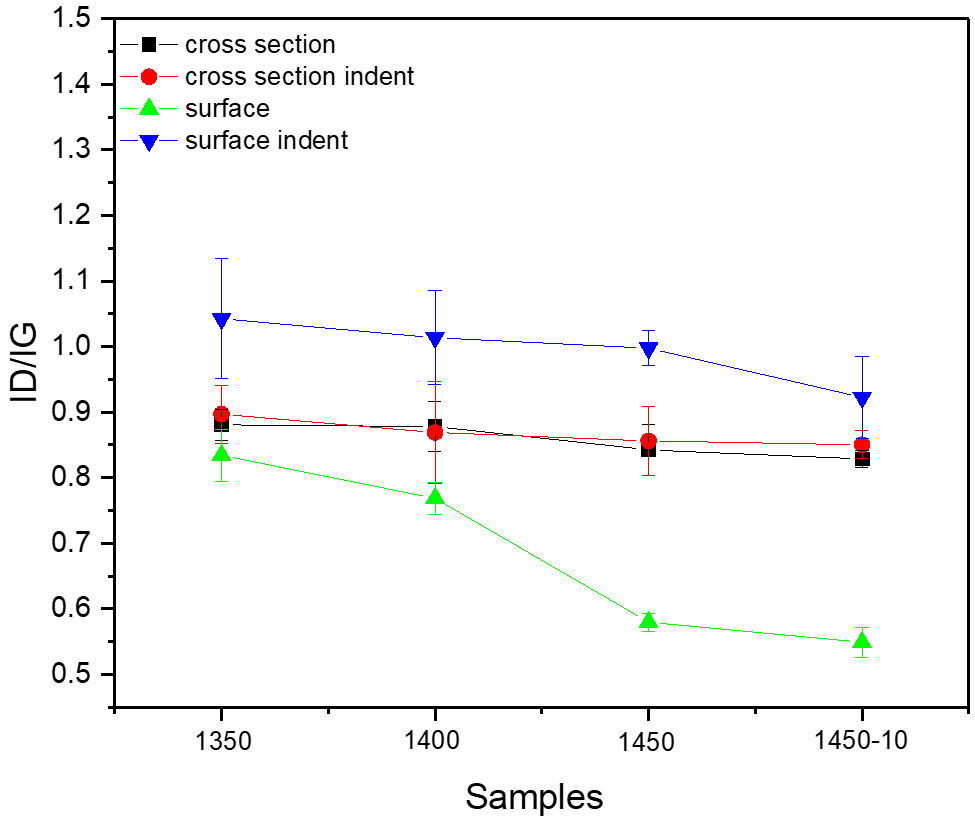
\includegraphics[width=0.7\textwidth]{Picture1.png}
	\caption{使用Tikz标注图片的例子}
	\label{fig:exam}
\end{figure}
首先我们要知道,使用命令来画图,必须要知道起始点与终点的坐标。那么如何在一张图片中确定坐标呢?而且这个坐标不能因为图片的缩放而改变。比较有效的一个方法就是以图片为坐标系,所以的坐标都是相对于图片而言的。这样我们就不怕图片的各种变化。\par
如何以图片为相对坐标系呢?可以使用\lstinline|\begin{scope}|来建立。有了坐标系,我们又如何确定画图起始点的坐标呢?一个一个点去试验嘛?当然可以。这是提供一种Will认为比较有效的方法,详细论述请见\href{https://tex.stackexchange.com/questions/9559/drawing-on-an-image-with-tikz}{此处}。简单来讲就是用helpline把坐标系给画出来,这样就知道具体的坐标,确认了坐标之后,再隐藏helpline。一段可用代码如下:
\begin{lstlisting}[language=TeX]
\begin{tikzpicture}
	\node[anchor=south west,inner sep=0] (image) at (0,0) {\includegraphics[width=0.9\textwidth]{some_image.jpg}};
	\begin{scope}[x={(image.south east)},y={(image.north west)}]
		\draw[help lines,xstep=.1,ystep=.1] (0,0) grid (1,1);
		\foreach \x in {0,1,...,9} { \node [anchor=north] at (\x/10,0) {0.\x}; }
		\foreach \y in {0,1,...,9} { \node [anchor=east] at (0,\y/10) {0.\y}; }
		%此处可以写入画图代码。
		\draw[red,ultra thick,rounded corners] (0.62,0.65) rectangle (0.78,0.75);
	\end{scope}
\end{tikzpicture}
\end{lstlisting}
根据这段代码我们可以实现如图\ref{fig:exam2}的效果。
\begin{figure}[h]
	\centering
	\begin{tikzpicture}
		\node[anchor=south west,inner sep=0](image) at (0,0) {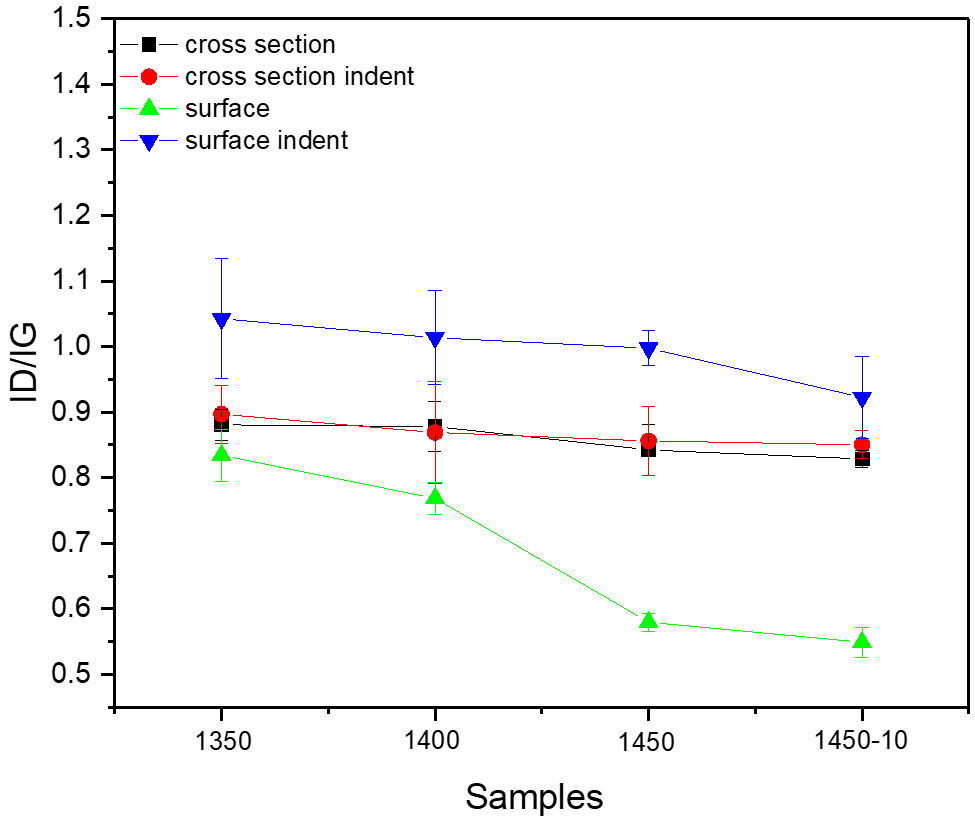
\includegraphics[width=0.7\textwidth]{Picture1.png}};
		\begin{scope}[x={(image.south east)},y={(image.north west)}]
			\draw[help lines, xstep=0.05, ystep=0.05](0,0) grid (1,1);
			\foreach \x in{0,1,...,9}{\node[anchor=north] at (\x/10,0) {0.\x};}
			\foreach \y in{0,1,...,9}{\node[anchor=east] at (0,\y/10) {0.\y};}
		\end{scope}
	\end{tikzpicture}
	\caption{使用helpline辅助确定坐标的例子}
	\label{fig:exam2}
\end{figure}

有了图\ref{fig:exam2},我们就可以确定起点坐标是\(0.2,0.43\),终点的坐标是\(0.9,0.53\)。有了这两个点我们就可以画一个包含红线与黑线的虚线框了。使用命令\lstinline|\draw[dashed,red,ultra thick,rounded corners] (0.2,0.43) rectangle (0.9,0.53);|。命令中dashed表示虚线,red代表红色,ultra thick是线宽,rounded corners则表示要画一个圆角框。具体的参数设置可以根据自己的需要参考文档说明确定。
\begin{note}
	使用Tikz宏包,不少时候需要再加载此宏包的一些预设库。比如要修改线型需要加载\lstinline|\usetikzlibrary{patterns}|。这些使用注意事项在文档中可以找到。
\end{note}

按照上面的各种操作确定坐标并且注释掉helpline等相关的代码之后,我们就可以得到图\ref{fig:exam3}的结果\footnote{不得不说,我们上面做了这么多的工作,才实现了在PPT中可以2-3秒完成的工作。每当此时,我都会陷入沉思 \faDizzy[regular]}。
\begin{figure}
	\centering
	\begin{tikzpicture}
	\node[anchor=south west,inner sep=0](image) at (0,0) {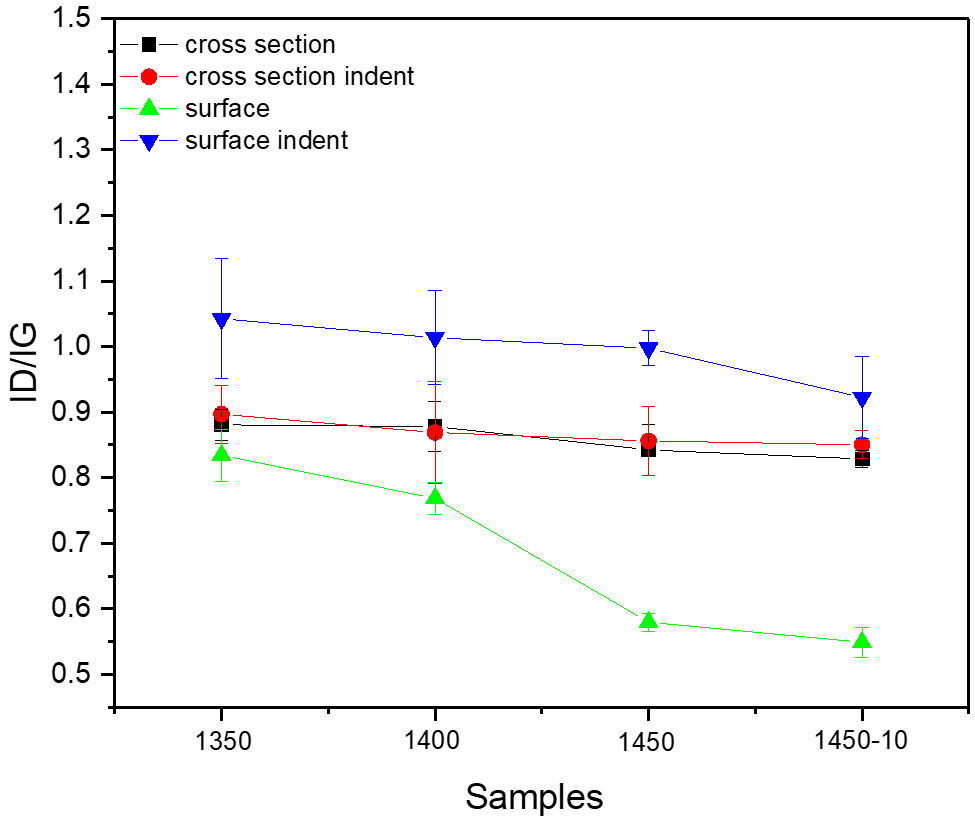
\includegraphics[width=0.7\textwidth]{Picture1.png}};
	\begin{scope}[x={(image.south east)},y={(image.north west)}]
	%\draw[help lines, xstep=0.05, ystep=0.05](0,0) grid (1,1);
	%\foreach \x in{0,1,...,9}{\node[anchor=north] at (\x/10,0) {0.\x};}
	%\foreach \y in{0,1,...,9}{\node[anchor=east] at (0,\y/10) {0.\y};}
	\draw[dashed,red,ultra thick,rounded corners] (0.2,0.43) rectangle (0.9,0.53);
	\end{scope}
	\end{tikzpicture}
	\caption{使用helpline辅助确定坐标的例子}
	\label{fig:exam3}
\end{figure}

\subsection{列表}
\label{par-list}
列表在PPT中绝对是极其重要的一个组件,尤其是在要列举各种观点、结论的时候。好的列表组织可以让人快速理解自己的想法\footnote{Will曾经见过有人把自己的结论“平铺”在一页PPT中,一眼看过去,眼花……}。我们知道列表分为有序列表与无序列表,在\LaTeX{} 中分别用itemize与enumerate表示无序与有序。列表作为一种基本的组件,其实并没有太多可以讲的。但是在PPT中,不仅需要提供内容,还需要提供一种便于听众理解、follow的形式。一旦需要对形式进行加工,那么需要操作的点无疑就多了起来:如何缩进,用什么符号、行距怎么设置。
\paragraph*{列表符号自定义}
有一个奇怪的现象,在PowerPoint进化到2019版的今天,虽然提供了几种默认并且相当好看的符号,PPT默认的列表符号还是让其看起来具有相当的时代感。一个小小的黑点实在让人难受。\LaTeX{} 同样也是默认这样一个小黑点。
\begin{itemize}
	\item 项目一
	\item 看看这个小黑点
\end{itemize}

如何对列表符号进行设置呢?在\LaTeX{} 的通常文档类中(article, book等)可以直接使用\lstinline|\renewcommand{\labelitemi}{def}|来重新定义。简单的例子如下\footnote{这条命令能否生效还要看你使用的文档类作者有没有进行魔改,比如在本文档使用的Eleagant文档类中就不生效}:

\begin{itemize}
	\item[\ding{118}] 项目一
	\item[\ding{118}] 新的项目符号
	\item[\ding{118}] 为了排版强加了第三行
\end{itemize}

但是在Beamer文档类中,就不能使用这种方法,而是应该按照beameruserguide中的建议使用如下的方式进行修改:
\begin{lstlisting}[language=TeX]
	\setbeamertemplate{itemize item}{\ding{118}} %后面的\ding{118}是我比较喜欢的一个符号
	\setbeamertemplate{itemize subitem}{} %二级列表
	\setbeamertemplate{itemize subsubitem}{} %三级列表
\end{lstlisting}

\paragraph*{列表分散对齐}
正常情况下,我们不需要对列表环境的对齐进行修改,只要使用默认的左对齐就可以了。但是在PPT中你就会发现列表大多数时间并不是单独列在一页上的(如是是这种情况也就不需要分散对齐),而是在一小块区域中列举出自己的几个结论。在英文的环境下,没有分散对齐,显得非常的难看。\par
\href{https://liam.page/2017/04/11/justifying-in-beamer-s-lists/}{此博文}\footnote{这位作者绝对是\LaTeX{} 的大神,但是对于其在文章中说只有处女座才会要求分散对齐的说法,本人持不同意见,技术应该是为人服务的,是为了实现人的需求的。PowerPoint就做的很好,给你特别高的自由度,你想怎么样,都可以简单的实现。}的作者给出了一种解决方法,使用xpatch宏包替换原Beamer文档类中的左对齐命令,从而可以实现分散对齐的要求。
\begin{lstlisting}[language=TeX]
\usepackage{ragged2e}
\usepackage{xpatch}
\xpatchcmd{\itemize}{\raggedright}{\justifying}{}{} %搜索并替换文档类中itemize中的\raggedright命令
\end{lstlisting}

\paragraph*{列表缩进与行距}
如果想要对列表进行如缩进,行距等设置,可以使用enumitem宏包,该宏包允许用户在itemize等环境后加跟参数,从而实现方便的定制。
\begin{note}
	在Beamer中,尽量不要使用enumitem宏包,使用了这个宏包之后需要面临很多模板(主题)方面的修改,比如\ref{par-list}小节中的列表符号自定义就要进行修改为enumitem item。 这个问题不会报错,所以你并不知道有宏包的冲突,你只会以纠结于得不到自己想要的结果。
\end{note}

在Beamer中如果只是简单的修改下列表的行距,使用\lstinline|\itemsep=**|就可以进行设置了。至于要修改全局的列表行距,可以参考此\link{https://tex.stackexchange.com/questions/16793/global-setting-of-spacing-between-items-in-itemize-environment-for-beamer}.
\section{标题}
对于标题的设置其实应该是由Beamer theme的作者进行的工作,通常不需要自己再去调整,我们只需要选用合适的theme,从而可以实现内容与样式的分离。多么美好的想法,但是这注定是行不通的。因为theme作者的水平参差不齐\footnote{只消去看下\href{https://www.overleaf.com/latex/templates/tagged/presentation/}{Overleaf}就知道现在的Beamer模板的质量},有的人能做到字体,版式,布局全部都好。但是有的人就只能做到一部分,而且绝大部分作者的theme都实在是一言难尽。所以我们可能还需要在原theme的基础上进行一系列修改,比如字体、字号、颜色、位置等等。
\subsection{标题字体、字号、颜色}
Beamer是一个与正常\LaTeX{} 文档类非常不同的文档类,重新定义了很多条目。最好的学习使用Beamer的方法就是去读beameruserguide\footnote{我至今没有读完\faSadCry[regular]},这个文档从初级使用到theme编写都写的很详细。在设定Beamer的字体、字号、颜色之前要首先知道自己设定的部分在Beamer中的“官方”名称。一个常见的设定方式如下:
\begin{lstlisting}[language=TeX]
	\setromanfont[Numbers=OldStyle]{Georgia}
	\setsansfont[Scale=MatchLowercase]{OpenSans} %设定rmfamily与sffamily
	\setbeamerfont{title}{family=\rmfamily,size=\huge, series=\bfseries} %不带星号表示追加参数
	\setbeamerfont*{subtitle}{size=\large, shape=\itshape} %带星号表示抹除之前的设定,重新按现在设定
	\setbeamerfont{section title}{size=\Large, series=\bfseries}
	\setbeamerfont{frametitle}{size=\large, series=\bfseries}
	\setbeamerfont{caption}{size=\footnotesize, series=\bfseries}
	\setbeamerfont{footnote}{size=\tiny}
	\setbeamerfont{alerted text}{series=\bfseries}
	\addtobeamertemplate{institute}{\raggedleft}{}%给模板中追加新的设定
	\setbeamercolor{normal text}{%设定颜色
	fg=black!2,
	bg=漆黑 %需要cncolours的支持,此theme未在CTAN发布
	}
\end{lstlisting}

从这个例子中,其实就可以看到,设定颜色、字号与字体比较直接。只需要定义family, size, series 与shape就可以。颜色的定义使用另外的\lstinline|\setbeamercolor{Beamer组件名称}{颜色}|进行设定。关于字体方面的内容可以参考第\ref{ch-1}章以及刘海洋《\LaTeX{} 入门》。
\subsection{标题位置}
对于标题位置的调整也比较直接,使用\lstinline|\setbeamertemplate{frametitle}{}|就可以。例子请见下方设置标题样式。
\begin{lstlisting}[language=TeX]
	\setbeamertemplate{title}{%
		\raggedleft
		\linespread{1.0}%
		\inserttitle
		\hspace*{1.2cm}\par
		\vspace*{0.5em}}%设定Beamer首页Title
	\setbeamertemplate{subtitle}{%
		\raggedleft
		\insertsubtitle
		\hspace*{1.2cm}\par
		\vspace*{0.5em}}%设定Beamer首页副标题
	\setbeamertemplate{title page}{
		\begin{minipage}[b]{\textwidth}
		\usebeamertemplate*{title graphic}\vfill
		\usebeamertemplate*{title}
		\usebeamertemplate*{subtitle}
		\usebeamertemplate*{title separator}
		\usebeamertemplate*{author}
		\usebeamertemplate*{date}
		\usebeamertemplate*{institute}
		\vfill
		\end{minipage}}%设定title page 组成
	\setbeamertemplate{frametitle}{\vskip0.06\paperheight\insertframetitle} %设置标题样式
\end{lstlisting}

\section{脚注、页码}
\subsection{页码}
页码这边的问题还有不少,其中一个重要的原因就是一些简单动画带来的:一个动画分为很多帧,每一帧在PDF中都是一页,但是这些页的页码应该是同一个页码。这就需要某些页不进行计数。当然还有其它问题,我们这里就例举一些最常见且实用的例子。
\paragraph*{页码样式}
页码样式无非就是罗马、阿拉伯、中文、中文大写等等吧,下面就展示下如何修改。
\begin{lstlisting}[language=TeX]
	\setbeamertemplate{frame numbering}{\zhnumber[style=Financial]{\insertframenumber}} %疑似来源于未记录的template
	%ctex文档类已经加载了zhnumber宏包,不需要再次加载。
\end{lstlisting}

这个例子中使用的template{frame numbering}未找到出处,在beameruserguide中也未检索到,怀疑是否是undocumented的条目\footnote{请见stone-zeng的项目\link{https://github.com/stone-zeng/latex-talk}}。\par
除了这种方式,还有另一种直接修改footline template的方法\footnote{这种方法中的\lstinline|\defbeamertemplate{}|,尤其是加星不加星到现在我也没搞清楚\faSadTear[regular]}。
\begin{lstlisting}[language=TeX]
	%设置 footline
	\defbeamertemplate*{footprogress}{UoM}
	{%
	\usebeamerfont{progress}\insertframenumber\ of \inserttotalframenumber}
	\defbeamertemplate*{footline}{UoM}
	{
	\ifx \insertframetitle \@empty
	% There was no frame title
	\else
	% There was a frame title, typeset the counterpart to the frame title (this is a hack).
	\begin{beamercolorbox}[sep=1\highsep,rightskip=1ex]{progress}%
	\phantom{ }
	\hfill
	\hbox{\usebeamertemplate{footprogress}}
	\end{beamercolorbox}%
	\fi
	}
\end{lstlisting}
\paragraph*{首页不编码}不少时候,我们不希望第一页的标题页进行编页,这个时候可以在frame环境后,加跟参数\textit{noframenumbering}来禁止此页编号。当此frame有标题时,\emph{参数要放在标题之前}。
\paragraph*{多页用同一页码}
balabala
\begin{lstlisting}[language=TeX]
\newcounter{continuationFirstSlide}
\setcounter{continuationFirstSlide}{1}

\setbeamertemplate{footline}{%
\ifnum\insertcontinuationcount>0 % decide is this a framebreak slide ("split frame"), if yes, decide whether its the first slide of the split or a continuation, if second, then reduce frame number by one to omit counting
\ifnum\thecontinuationFirstSlide=1
\setcounter{continuationFirstSlide}{0}
\else
\addtocounter{framenumber}{-1}
\fi
\else % no continuation, so the next framebreak slide is a first slide, that gets a new number
\setcounter{continuationFirstSlide}{1}
\fi
\insertframenumber/\inserttotalframenumber
}
\begin{document}
\frame{}
\begin{frame}[allowframebreaks]
abc
\framebreak
XYZ
\end{frame}
\frame{last frame}
\end{document}
\end{lstlisting}
\paragraph*{PDF书签设置}
因为有时候会产生\textit{allowframebreaks}的情况,比如\lstinline|\pause|等,此时如果要生成合理的PDF书签,则需要特别的设置。一个非常好的解答请见\link{https://tex.stackexchange.com/questions/203127/beamer-bookmarks-with-allowframbreaks}。 我也摘录在下面:
\begin{lstlisting}[language=TeX]
\apptocmd{\beamer@@frametitle}{%
\only<1>{\bookmark[page=\the\c@page,level=3]{#1 \expandafter\ifnum\insertcontinuationcount>0\relax\insertcontinuationcount\fi}}}% 分页之后连编号并加入书签
\apptocmd{\beamer@@frametitle}{%
\only<1>{\expandafter\ifnum\insertcontinuationcount<2\relax\bookmark[page=\the\c@page,level=3]{#1}\fi}}%只第一页加入书签
\end{lstlisting}

\end{document}
